\subsubsection{Kinetic-energy consistency of MPAS-O $\rightarrow$ ROMS remapping}
%{Niskine, Gulf Stream, Bay of Bengal and Chesapeake Bay test cases}

One of the primary tests in determining whether the complex remapping procedure yields consistent and accurate solutions is to evaluate whether the kinetic energy (KE) of the MPAS-O daily-mean solution survives the solution transfer to the \ROMS grids. For each of the daily average snapshots in the 2-month dataset used here, the KE is computed on the \MPAS cells and on the \ROMS grid with exact area weights and fractions that have been computed using a fully conservative map. Using this linear map, the surface average KE and depth averaged KE at various levels are calculated and compared.

Let $A_a,f_a$ be the area and covered fraction of MPAS cell $a$, and $A_b,f_b$ those of ROMS rho cell $b$. If the weights are given as $w_a=f_aA_a$ and $w_b=f_bA_b\,\chi_b$, where $\chi_b=1$ on ocean cells and $0$ on land, then we can define the following metrics for verification.


On MPAS, $u,v$ represent the zonal and the meridional velocity components,  and on ROMS, these are the face velocities that are averaged to cell centers (masked land faces are ignored). The surface kinetic energy metric used in this study and as shown in Fig.~\ref{fig:region_KE} is defined by
\begin{equation}
	\mathrm{KE}=\frac{1}{2}\left(u^2+v^2\right)\quad [\si{\metre\squared\per\second\squared}],
	\label{conv:eq:ke}
\end{equation}
with velocities represented at cell centers for the diagnostic.

\textbf{Kinetic energy per unit mass:} 
%
This is derived as a simple metric is to eliminate the thickness of the top surface layer and instead use the following:
\begin{equation}
	\langle \mathrm{KE}\rangle_{\rm surf}=\frac{\sum_a w_a\,\mathrm{KE}^a_{0}}{\sum_a w_a}\quad\text{vs.}\quad \frac{\sum_b w_b\,\mathrm{KE}^b_{\rm top}}{\sum_b w_b}.
\end{equation}

This yeilds the average surface KE per unit mass at the ocean surface. 

\textbf{Depth-clipped integrals:}
%
In a column with layer thicknesses $\Delta z_k$ ($k=0$ at the surface), the depth of the layer top is $d_k=\sum_{j<k}\Delta z_j$ and the part of layer $k$ above depth $D$ is $\omega_k(D)=\min\!\big[\max(D-d_k,0),\,\Delta z_k\big]$. Then
\begin{equation}
I_{\rm MPAS}(D)=\sum_a w_a\sum_k\omega^{a}_k(D)\,\mathrm{KE}^{a}_k,\qquad
I_{\rm ROMS}(D)=\sum_b w_b\sum_k\omega^{b}_k(D)\,\mathrm{KE}^{b}_k ,
\end{equation}
with $D=50$, $100$~m and $D=\infty$ (full column, ``global'' integral) for all cases except for Chesapeake Bay. Here, we choose $D=10,20$~m since most of the estuary region have a  maximum depth of 38m. 


\textbf{Conservative-map reference.} As a standard reference, we also compare the fully conservative linear sparse map operator that computes the projection of the MPAS surface velocities as a SpMV product. Then $\langle\mathrm{KE}\rangle_{\rm surf}=\sum_b w_b\tfrac12(u_b^2+v_b^2)/\sum_b w_b$, provides the horizontal conservative remap of surface KE that can be compared against the bilinear variant.


%\begin{table}
%\small
%\begin{tabular}{lcccccc}\toprule
% & Surface & Top 50\,m$^\dagger$ & Top 100\,m$^\dagger$ & Full depth & Cons.-map surface\\\midrule
%Niskine        & $-5.5$ to $-4.9$ & $-2.7$ to $-2.4$ & $-2.4$ to $-2.1$ & $-2.1$ to $-1.8$ & $-0.35$ to $-0.29$\\
%Gulf Stream    & $-1.4$ to $-1.1$ & $-1.4$ to $-1.1$ & $-1.3$ to $-1.1$ & $-1.2$ to $-1.0$ & $-0.27$ to $-0.21$\\
%Bay of Bengal  & $-1.7$ to $-1.6$ & $-1.6$ to $-1.4$ & $-1.7$ to $-1.6$ & $-2.0$ to $-1.9$ & $-0.55$ to $-0.51$\\
%Chesapeake Bay & $-11$ to $-6$ & $-23$ to $-4$ & $-21$ to $-4$ & $-20$ to $-5$ & $-1.3$ to $-0.7$\\\bottomrule
%\end{tabular}\\[2pt]
%\caption{Range over time of $100\,(\mathrm{ROMS}/\mathrm{MPAS}-1)$ in \%. $^\dagger$10\,m and 20\,m for Chesapeake.}
%\end{table}


\begin{figure}[htbp]
	\centering
	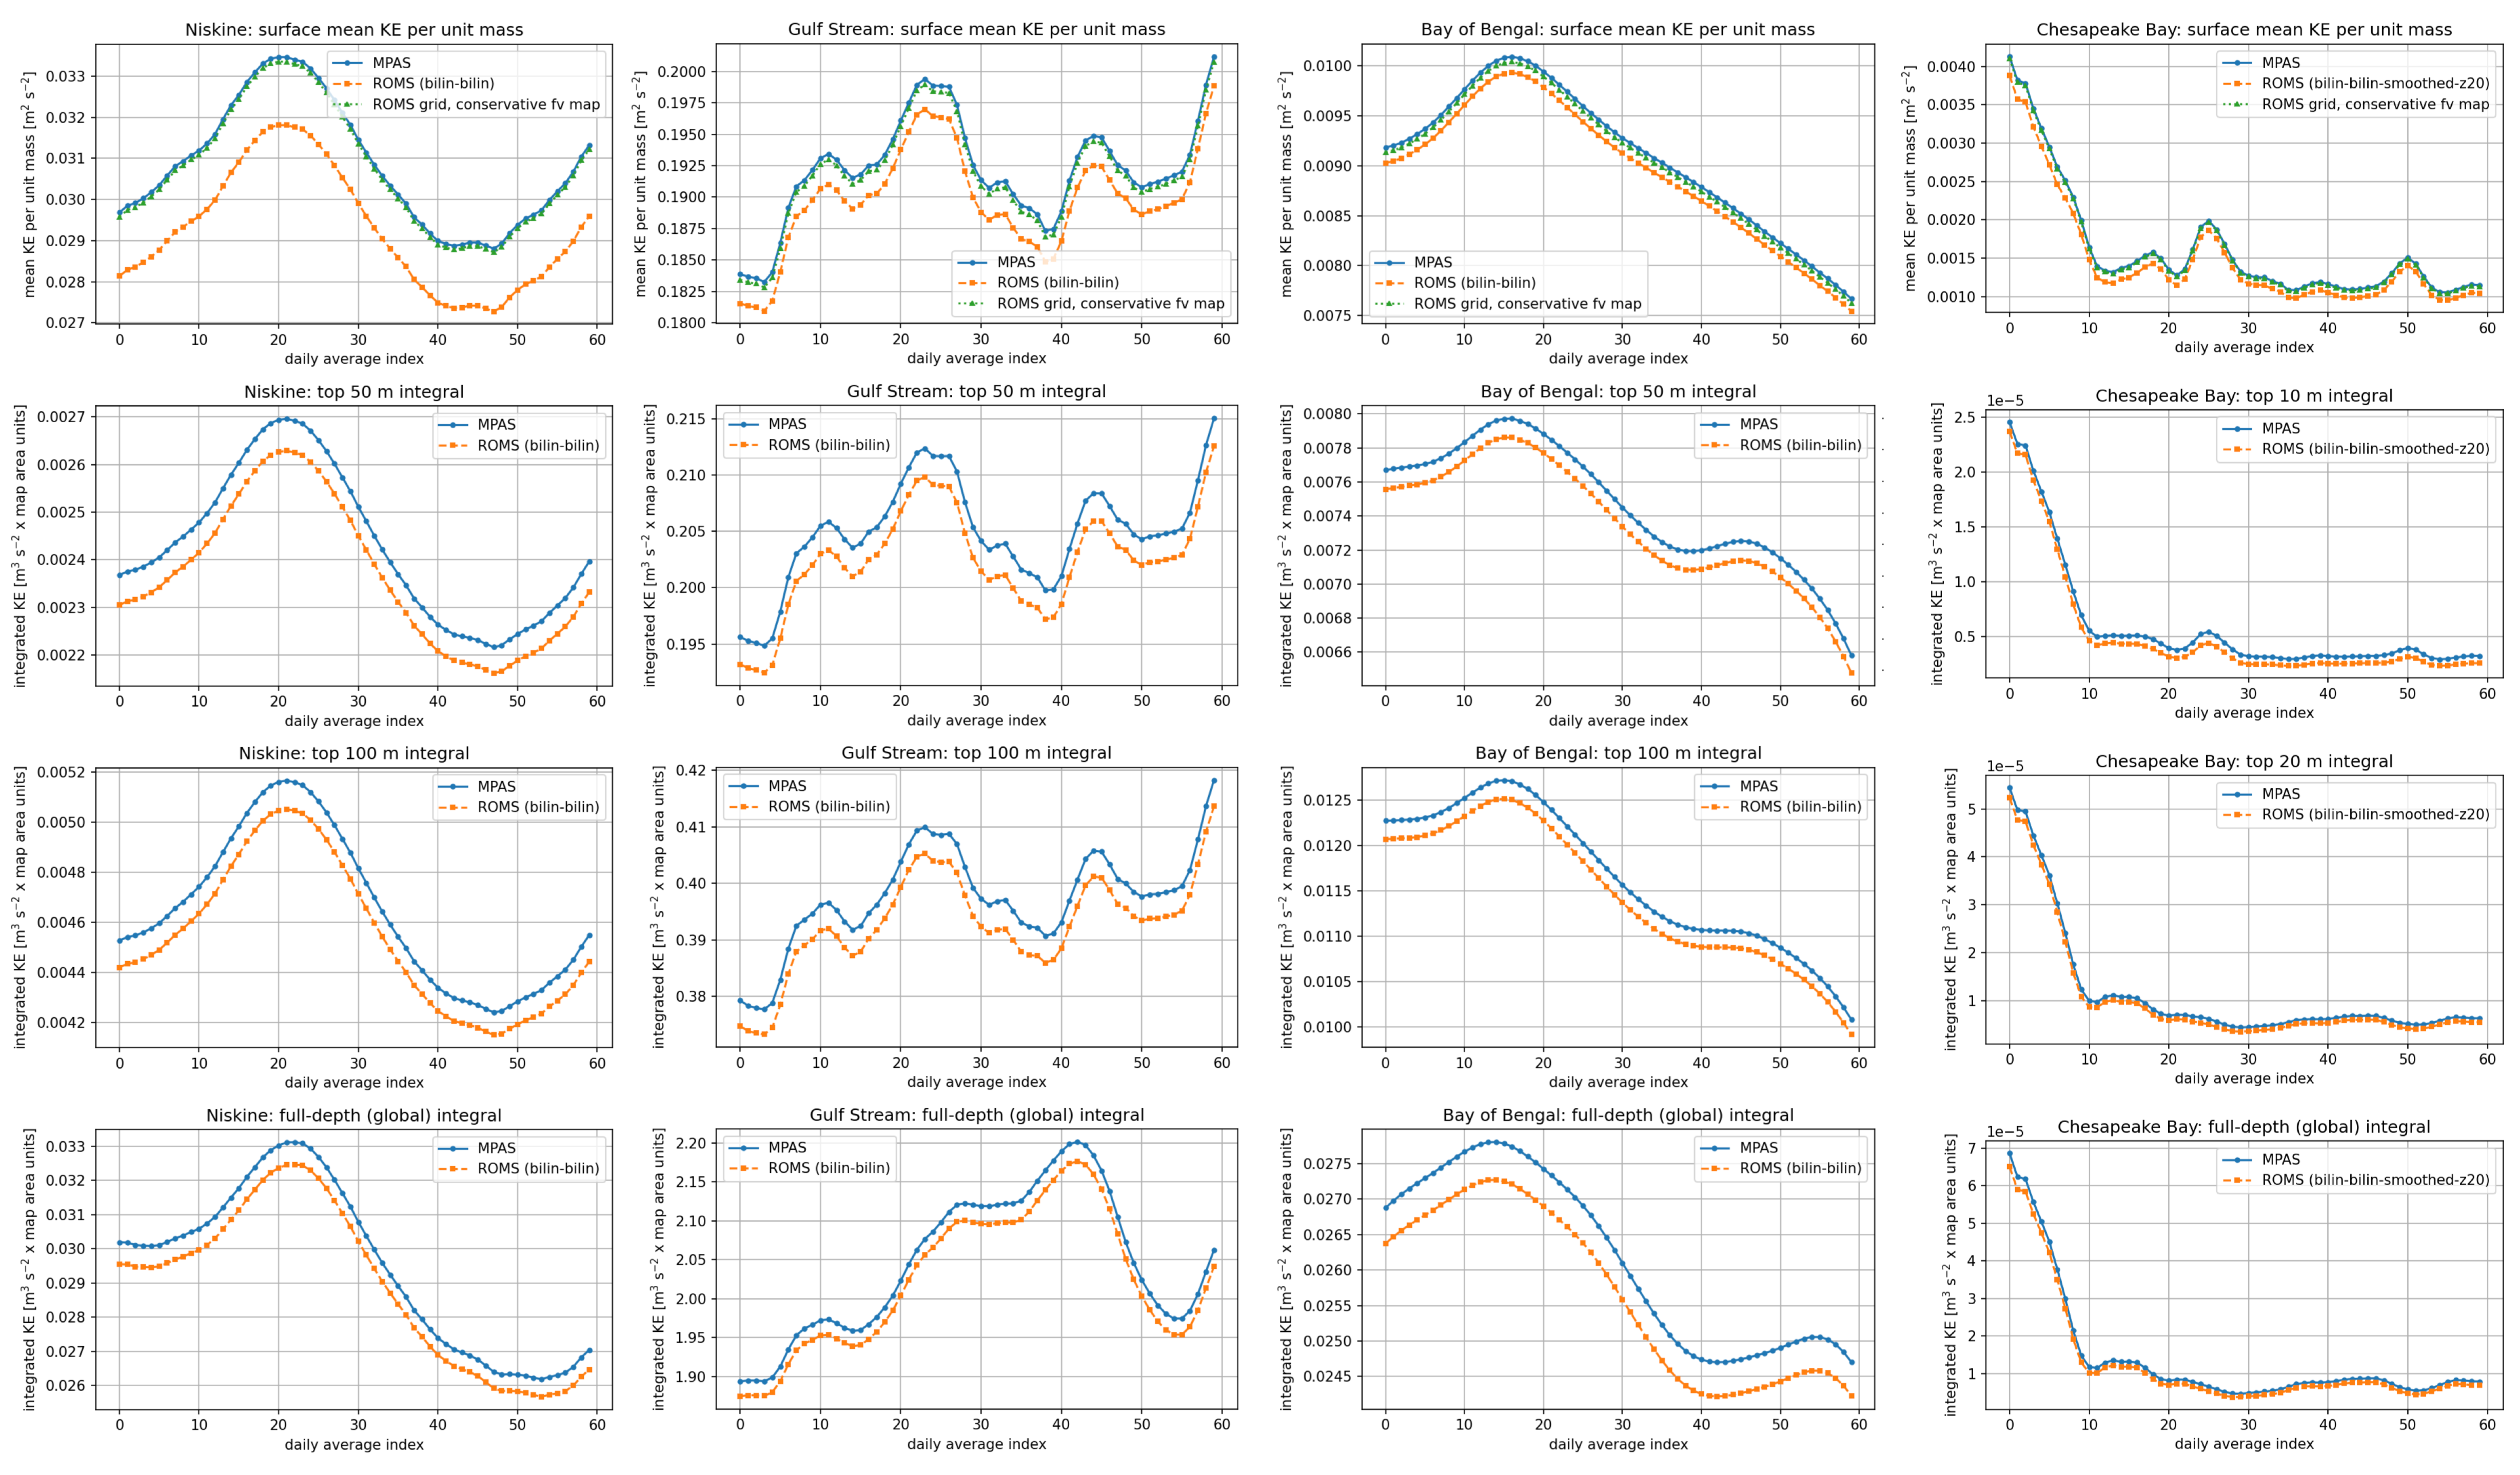
\includegraphics[width=\textwidth]{Figures/regional_KEmetrics_alldomains.png}
  \caption{Kinetic-energy time series for NISKINe, the Gulf Stream, the Bay of Bengal, and Chesapeake Bay.}
	\label{fig:region_KE}
\end{figure}


The metrics profiles as demonstrated in Fig.~\ref{fig:region_KE} show that the remapped \ROMS solution holds 95--99\% of the \MPAS KE, with the same time evolution, and the deficit is remains nearly constant in time i.e., spatial remapping error is decoupled. The depth-integrated and full-column KE values are within a 2\% agreement range. Only the Niskine domain has the largest surface deficit of about 5\% \TODOc{investigate further}. We also note that for regional domains, the surface deficit exceeds the depth integrated ones as the \ROMS SSH and top surface are generally shallower, while the \MPAS fixed z-coordinate top level layer is almost twice as deep. This contributes to the surface mean KE discrepancy. Deeper layers contribute less KE per metre, and hence the integral is less sensitive to any transfer errors.

We also compared a fully conservative map, which remains within 0.5\% in all cases. The difference includes the expected Jensen loss because $\overline{u}^2\le\overline{u^2}$ over a \ROMS cell. It also includes regions where the higher-resolution \ROMS bottom cells extend slightly below the \MPAS bottom depth.
%
For the coastal regional domains specifically, after carefully imposing the same \MPAS land masking onto \ROMS, the Bay of Bengal domain (with about 15\% land cells) is no worse than the open-ocean cases.  Validating the Chesapeake Bay region was especially harder since the domain is much shallower with over 65\% land masked cells at 600~m resolution, and with a coastline far finer than the MPAS cells. Due to the specific domain setup, the KE in the flow is much smaller, which results in lower absolute error propagation at the cutoff boundary where the solution is blended with conditions from a standalone regional simulation. \TODOc{reference Kyle's previous note}

%\FloatBarrier

%The Gulf Stream and Bay of Bengal applications use shared-area characteristic-length ratios $\hRatio\approx0.23$ and $0.29$, respectively. In every domain the regional solution alters both the geometry of the flow and its energy content relative to the \MPAS state. Because the regional model continues to evolve after initialization, these differences measure the combined effect of the transfer and the subsequent regional dynamics, and the convergence experiments of Sect.~\ref{conv:sec:conv} remain the quantitative statement about the transfer itself. {\color{red} The Chesapeake result depends particularly strongly on native bathymetry, land-mask treatment, and the blended estuarine fields, and we regard it as preliminary: the blending procedure is not specified in enough detail here for the case to be reproduced exactly. }
%\TODOc{Kyle: not entire sure if the above paragraph sits well here}
